\documentclass[tikz,border=4pt]{standalone}
\usepackage{amsmath}
\usepackage{tikz}
\usepackage{circuitikz}
\usetikzlibrary{arrows.meta,positioning,calc,shapes.geometric,fit}

\begin{document}
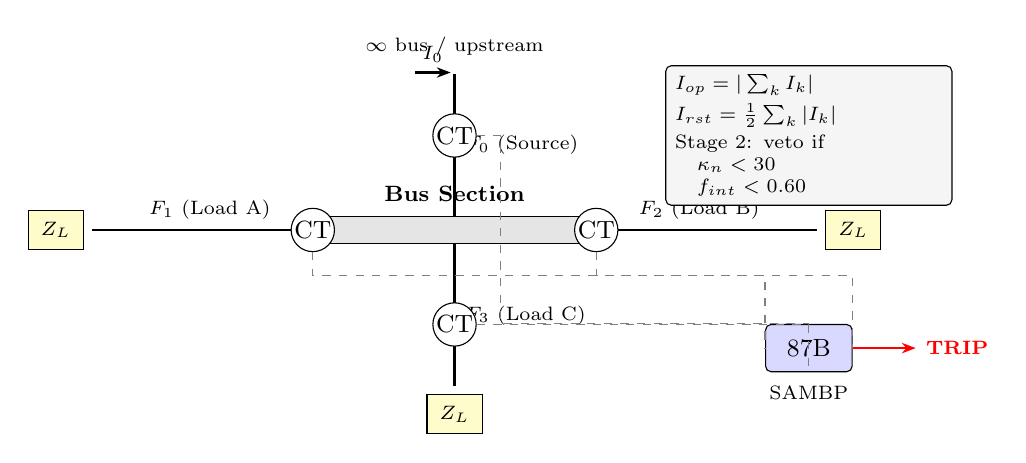
\begin{tikzpicture}[
  font=\small,
  bus/.style={draw,fill=gray!20,minimum width=3.2cm,minimum height=0.35cm},
  ct/.style={draw,circle,minimum size=0.55cm,fill=white,inner sep=0pt},
  relay/.style={draw,rectangle,minimum width=1.1cm,minimum height=0.6cm,
                fill=blue!15,rounded corners=2pt},
  feeder/.style={draw,thick},
  arr/.style={-{Stealth[length=5pt]},thick},
  label_style/.style={font=\scriptsize},
]

%% ===== Bus bar ===============================================================
\node[bus] (bus) at (0,0) {};
\node[above=0.05cm of bus,font=\footnotesize\bfseries] {Bus Section};

%% ===== Feeder 0: Source (top) ================================================
\draw[feeder] (bus.north) -- ++(0, 1.8) node[midway,right,label_style]{$F_0$ (Source)};
\node[ct] (ct0) at (0, 1.2) {CT};
\draw[arr] (-0.5,2.0) -- node[above,label_style]{$I_0$} (-0.05,2.0);
\node[above=1.9cm of bus,font=\scriptsize] {$\infty$ bus / upstream};

%% ===== Feeder 1: Load A (left) ===============================================
\draw[feeder] (bus.west) -- ++(-3.0, 0) node[midway,above,label_style]{$F_1$ (Load A)};
\node[ct] (ct1) at (-1.8, 0) {CT};
\node[left=3.1cm of bus,draw,fill=yellow!20,minimum width=0.7cm,
      minimum height=0.5cm,font=\scriptsize] (ld1) {$Z_L$};

%% ===== Feeder 2: Load B (right) =============================================
\draw[feeder] (bus.east) -- ++(3.0, 0) node[midway,above,label_style]{$F_2$ (Load B)};
\node[ct] (ct2) at (1.8, 0) {CT};
\node[right=3.1cm of bus,draw,fill=yellow!20,minimum width=0.7cm,
      minimum height=0.5cm,font=\scriptsize] (ld2) {$Z_L$};

%% ===== Feeder 3: Load C (bottom) ============================================
\draw[feeder] (bus.south) -- ++(0,-1.8) node[midway,right,label_style]{$F_3$ (Load C)};
\node[ct] (ct3) at (0,-1.2) {CT};
\node[below=1.9cm of bus,draw,fill=yellow!20,minimum width=0.7cm,
      minimum height=0.5cm,font=\scriptsize] (ld3) {$Z_L$};

%% ===== 87B Relay =============================================================
\node[relay] (relay) at (4.5, -1.5) {87B};
\node[below=0.05cm of relay,label_style] {SAMBP};

%% ===== CT wiring to relay ====================================================
\draw[dashed,gray] (ct0.east) -- ++(0.3,0) |- (relay.north);
\draw[dashed,gray] (ct1.south) -- ++(0,-0.3) -| (relay.west);
\draw[dashed,gray] (ct2.south) -- ++(0,-0.3) -| (relay.east);
\draw[dashed,gray] (ct3.east)  -- ++(0.3,0) -| (relay.south);

%% ===== Trip output ===========================================================
\draw[arr,red,thick] (relay.east) -- ++(0.8,0)
  node[right,font=\scriptsize,red]{\textbf{TRIP}};

%% ===== Equations annotation ==================================================
\node[draw,rounded corners=2pt,fill=gray!8,align=left,font=\scriptsize,
      text width=3.4cm] at (4.5, 1.2) {
  $I_{op} = |\sum_k I_k|$\\[2pt]
  $I_{rst} = \tfrac{1}{2}\sum_k |I_k|$\\[2pt]
  Stage 2: veto if\\
  \quad $\kappa_n < 30$\\
  \quad $f_{int} < 0.60$
};

\end{tikzpicture}
\end{document}
